\documentclass[tikz,border=10pt]{standalone}
% calc is needed for the $(E)+(...)$ coordinate arithmetic in the right-angle mark
\usetikzlibrary{calc}
\begin{document}
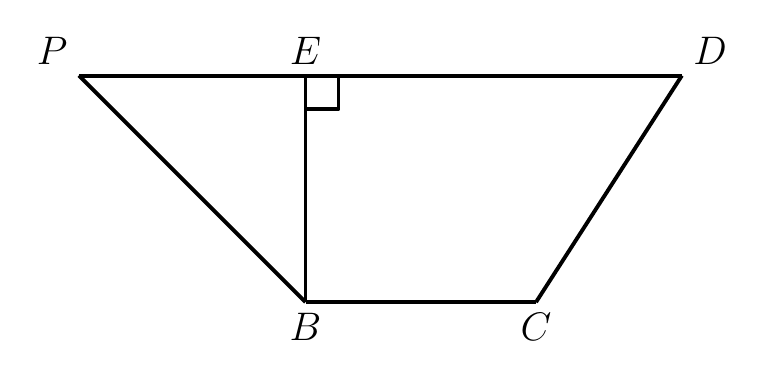
\begin{tikzpicture}[line join=round, line width=1.6pt]
  % Coordinates unchanged: s = 0.01626 cm/px, centred on ink bbox (cx=282.5, cy=153.5), y flipped
  \coordinate (P) at (-3.829, 1.439);
  \coordinate (E) at (-0.951, 1.439);
  \coordinate (D) at ( 3.829, 1.439);
  \coordinate (B) at (-0.951,-1.439);
  \coordinate (C) at ( 1.976,-1.439);

  % Segments: P-D (through E), P-B, E-B, B-C, C-D; stroke 1.4pt on these five
  \draw[line width=1.4pt] (P) -- (D);
  \draw[line width=1.4pt] (P) -- (B);
  \draw[line width=1.4pt] (E) -- (B);
  \draw[line width=1.4pt] (B) -- (C);
  \draw[line width=1.4pt] (C) -- (D);

  % Right-angle mark at E (between ED and EB), unchanged, line width 1.2pt
  \draw[line width=1.2pt] ($(E)+(0.423,0)$) -- ($(E)+(0.423,-0.423)$) -- ($(E)+(0,-0.423)$);

  % Point labels: plain math italic, \Large, same anchors as before
  \node[above left,  font=\Large] at (P) {$P$};
  \node[above,       font=\Large] at (E) {$E$};
  \node[above right, font=\Large] at (D) {$D$};
  \node[below,       font=\Large] at (B) {$B$};
  \node[below,       font=\Large] at (C) {$C$};
\end{tikzpicture}
\end{document}